\documentclass[twoside]{book}

% Packages required by doxygen
\usepackage{fixltx2e}
\usepackage{calc}
\usepackage{doxygen}
\usepackage[export]{adjustbox} % also loads graphicx
\usepackage{graphicx}
\usepackage[utf8]{inputenc}
\usepackage{makeidx}
\usepackage{multicol}
\usepackage{multirow}
\PassOptionsToPackage{warn}{textcomp}
\usepackage{textcomp}
\usepackage[nointegrals]{wasysym}
\usepackage[table]{xcolor}

% Font selection
\usepackage[T1]{fontenc}
\usepackage[scaled=.90]{helvet}
\usepackage{courier}
\usepackage{amssymb}
\usepackage{sectsty}
\renewcommand{\familydefault}{\sfdefault}
\allsectionsfont{%
  \fontseries{bc}\selectfont%
  \color{darkgray}%
}
\renewcommand{\DoxyLabelFont}{%
  \fontseries{bc}\selectfont%
  \color{darkgray}%
}
\newcommand{\+}{\discretionary{\mbox{\scriptsize$\hookleftarrow$}}{}{}}

% Page & text layout
\usepackage{geometry}
\geometry{%
  a4paper,%
  top=2.5cm,%
  bottom=2.5cm,%
  left=2.5cm,%
  right=2.5cm%
}
\tolerance=750
\hfuzz=15pt
\hbadness=750
\setlength{\emergencystretch}{15pt}
\setlength{\parindent}{0cm}
\setlength{\parskip}{0.2cm}
\makeatletter
\renewcommand{\paragraph}{%
  \@startsection{paragraph}{4}{0ex}{-1.0ex}{1.0ex}{%
    \normalfont\normalsize\bfseries\SS@parafont%
  }%
}
\renewcommand{\subparagraph}{%
  \@startsection{subparagraph}{5}{0ex}{-1.0ex}{1.0ex}{%
    \normalfont\normalsize\bfseries\SS@subparafont%
  }%
}
\makeatother

% Headers & footers
\usepackage{fancyhdr}
\pagestyle{fancyplain}
\fancyhead[LE]{\fancyplain{}{\bfseries\thepage}}
\fancyhead[CE]{\fancyplain{}{}}
\fancyhead[RE]{\fancyplain{}{\bfseries\leftmark}}
\fancyhead[LO]{\fancyplain{}{\bfseries\rightmark}}
\fancyhead[CO]{\fancyplain{}{}}
\fancyhead[RO]{\fancyplain{}{\bfseries\thepage}}
\fancyfoot[LE]{\fancyplain{}{}}
\fancyfoot[CE]{\fancyplain{}{}}
\fancyfoot[RE]{\fancyplain{}{\bfseries\scriptsize Generated on Mon Nov 16 2015 15\+:34\+:29 for My Project by Doxygen }}
\fancyfoot[LO]{\fancyplain{}{\bfseries\scriptsize Generated on Mon Nov 16 2015 15\+:34\+:29 for My Project by Doxygen }}
\fancyfoot[CO]{\fancyplain{}{}}
\fancyfoot[RO]{\fancyplain{}{}}
\renewcommand{\footrulewidth}{0.4pt}
\renewcommand{\chaptermark}[1]{%
  \markboth{#1}{}%
}
\renewcommand{\sectionmark}[1]{%
  \markright{\thesection\ #1}%
}

% Indices & bibliography
\usepackage{natbib}
\usepackage[titles]{tocloft}
\setcounter{tocdepth}{3}
\setcounter{secnumdepth}{5}
\makeindex

% Hyperlinks (required, but should be loaded last)
\usepackage{ifpdf}
\ifpdf
  \usepackage[pdftex,pagebackref=true]{hyperref}
\else
  \usepackage[ps2pdf,pagebackref=true]{hyperref}
\fi
\hypersetup{%
  colorlinks=true,%
  linkcolor=blue,%
  citecolor=blue,%
  unicode%
}

% Custom commands
\newcommand{\clearemptydoublepage}{%
  \newpage{\pagestyle{empty}\cleardoublepage}%
}


%===== C O N T E N T S =====

\begin{document}

% Titlepage & ToC
\hypersetup{pageanchor=false,
             bookmarks=true,
             bookmarksnumbered=true,
             pdfencoding=unicode
            }
\pagenumbering{roman}
\begin{titlepage}
\vspace*{7cm}
\begin{center}%
{\Large My Project }\\
\vspace*{1cm}
{\large Generated by Doxygen 1.8.10}\\
\vspace*{0.5cm}
{\small Mon Nov 16 2015 15:34:29}\\
\end{center}
\end{titlepage}
\clearemptydoublepage
\tableofcontents
\clearemptydoublepage
\pagenumbering{arabic}
\hypersetup{pageanchor=true}

%--- Begin generated contents ---
\chapter{S\+E\+N\+G330-\/assignment-\/2}
\label{md__r_e_a_d_m_e}
\hypertarget{md__r_e_a_d_m_e}{}
\input{md__r_e_a_d_m_e}
\chapter{Hierarchical Index}
\section{Class Hierarchy}
This inheritance list is sorted roughly, but not completely, alphabetically\+:\begin{DoxyCompactList}
\item \contentsline{section}{Equipment}{\pageref{class_equipment}}{}
\begin{DoxyCompactList}
\item \contentsline{section}{Bowflex}{\pageref{class_bowflex}}{}
\item \contentsline{section}{Treadmill}{\pageref{class_treadmill}}{}
\end{DoxyCompactList}
\item \contentsline{section}{Equipment\+Manager}{\pageref{class_equipment_manager}}{}
\end{DoxyCompactList}

\chapter{Class Index}
\section{Class List}
Here are the classes, structs, unions and interfaces with brief descriptions\+:\begin{DoxyCompactList}
\item\contentsline{section}{\hyperlink{class_bowflex}{Bowflex} }{\pageref{class_bowflex}}{}
\item\contentsline{section}{\hyperlink{class_equipment}{Equipment} }{\pageref{class_equipment}}{}
\item\contentsline{section}{\hyperlink{class_equipment_manager}{Equipment\+Manager} }{\pageref{class_equipment_manager}}{}
\item\contentsline{section}{\hyperlink{class_treadmill}{Treadmill} }{\pageref{class_treadmill}}{}
\end{DoxyCompactList}

\chapter{Class Documentation}
\hypertarget{class_bowflex}{}\section{Bowflex Class Reference}
\label{class_bowflex}\index{Bowflex@{Bowflex}}
Inheritance diagram for Bowflex\+:\begin{figure}[H]
\begin{center}
\leavevmode
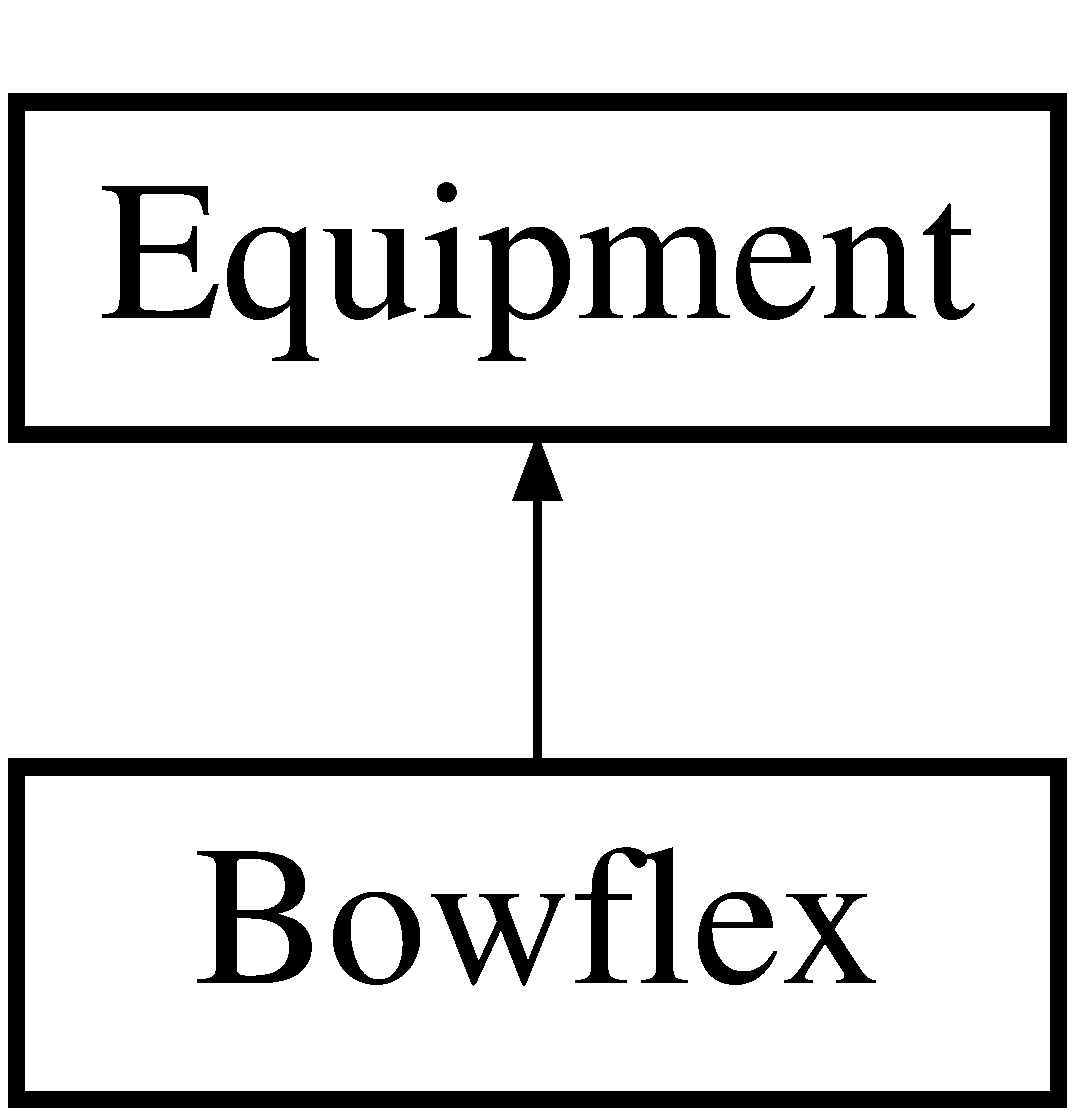
\includegraphics[height=2.000000cm]{class_bowflex}
\end{center}
\end{figure}
\subsection*{Public Member Functions}
\begin{DoxyCompactItemize}
\item 
\hypertarget{class_bowflex_aedb784e8d6845101938ec489f52627b7}{}{\bfseries Bowflex} (string in\+Brand)\label{class_bowflex_aedb784e8d6845101938ec489f52627b7}

\item 
\hypertarget{class_bowflex_a6a28e3b55ad31c4cc4df779d7f0377ab}{}\hyperlink{class_bowflex}{Bowflex} $\ast$ \hyperlink{class_bowflex_a6a28e3b55ad31c4cc4df779d7f0377ab}{clone} () const \label{class_bowflex_a6a28e3b55ad31c4cc4df779d7f0377ab}

\begin{DoxyCompactList}\small\item\em Create a clone of this piece of equipment at the same state. \end{DoxyCompactList}\item 
\hypertarget{class_bowflex_aa80bbb6167cbc96a85c4c251f7bd4322}{}string \hyperlink{class_bowflex_aa80bbb6167cbc96a85c4c251f7bd4322}{to\+String} () const \label{class_bowflex_aa80bbb6167cbc96a85c4c251f7bd4322}

\begin{DoxyCompactList}\small\item\em Return a string representation of this piece of equipment, in this case \textquotesingle{}\hyperlink{class_bowflex}{Bowflex}\textquotesingle{}. \end{DoxyCompactList}\item 
\hypertarget{class_bowflex_a6dacc10859384c1fb25f0832c63c5962}{}virtual void \hyperlink{class_bowflex_a6dacc10859384c1fb25f0832c63c5962}{serialize} (std\+::ostream \&os) const \label{class_bowflex_a6dacc10859384c1fb25f0832c63c5962}

\begin{DoxyCompactList}\small\item\em Serialize this piece of equipment as J\+S\+O\+N. \end{DoxyCompactList}\end{DoxyCompactItemize}
\subsection*{Additional Inherited Members}


The documentation for this class was generated from the following file\+:\begin{DoxyCompactItemize}
\item 
main.\+cpp\end{DoxyCompactItemize}

\hypertarget{class_equipment}{}\section{Equipment Class Reference}
\label{class_equipment}\index{Equipment@{Equipment}}


{\ttfamily \#include $<$Equipment.\+h$>$}

Inheritance diagram for Equipment\+:\begin{figure}[H]
\begin{center}
\leavevmode
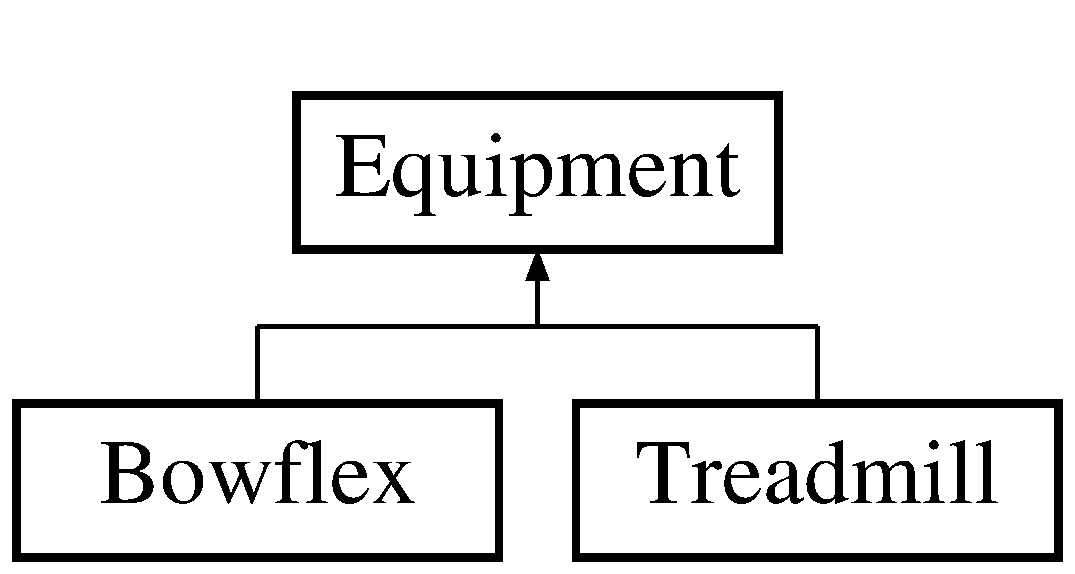
\includegraphics[height=2.000000cm]{class_equipment}
\end{center}
\end{figure}
\subsection*{Public Member Functions}
\begin{DoxyCompactItemize}
\item 
\hypertarget{class_equipment_a5c6929939d117e84e182e21a62a7723a}{}virtual \hyperlink{class_equipment}{Equipment} $\ast$ \hyperlink{class_equipment_a5c6929939d117e84e182e21a62a7723a}{clone} () const  =0\label{class_equipment_a5c6929939d117e84e182e21a62a7723a}

\begin{DoxyCompactList}\small\item\em Create a clone of this piece of equipment at the same state. \end{DoxyCompactList}\item 
\hypertarget{class_equipment_a970f5be54182c0067cb2cbb72c0029b6}{}virtual std\+::string \hyperlink{class_equipment_a970f5be54182c0067cb2cbb72c0029b6}{to\+String} () const  =0\label{class_equipment_a970f5be54182c0067cb2cbb72c0029b6}

\begin{DoxyCompactList}\small\item\em Return a string representation of this piece of equipment. \end{DoxyCompactList}\item 
\hypertarget{class_equipment_adc36912d637c7c445db05cab803abeb3}{}virtual void \hyperlink{class_equipment_adc36912d637c7c445db05cab803abeb3}{serialize} (std\+::ostream \&os) const  =0\label{class_equipment_adc36912d637c7c445db05cab803abeb3}

\begin{DoxyCompactList}\small\item\em Serialize the equipment as J\+S\+O\+N. \end{DoxyCompactList}\item 
\hypertarget{class_equipment_a7547b5114f15bb1bdc4ddc1c14da3c8d}{}virtual \hyperlink{class_equipment_a7547b5114f15bb1bdc4ddc1c14da3c8d}{$\sim$\+Equipment} ()\label{class_equipment_a7547b5114f15bb1bdc4ddc1c14da3c8d}

\begin{DoxyCompactList}\small\item\em Set the brand. \end{DoxyCompactList}\item 
\hypertarget{class_equipment_a15b661908f1f70cb15e910d59c879b01}{}virtual void \hyperlink{class_equipment_a15b661908f1f70cb15e910d59c879b01}{set\+Brand} (std\+::string in\+Brand)\label{class_equipment_a15b661908f1f70cb15e910d59c879b01}

\begin{DoxyCompactList}\small\item\em Set the brand of equipment. \end{DoxyCompactList}\item 
\hypertarget{class_equipment_adf98a9485c7dd511ee55b34e328f2eb0}{}virtual std\+::string \hyperlink{class_equipment_adf98a9485c7dd511ee55b34e328f2eb0}{get\+Brand} ()\label{class_equipment_adf98a9485c7dd511ee55b34e328f2eb0}

\begin{DoxyCompactList}\small\item\em Get the brand of equipment. \end{DoxyCompactList}\item 
\hypertarget{class_equipment_ad353e0121f958ee31f56ef7a7b4ff1e0}{}virtual void \hyperlink{class_equipment_ad353e0121f958ee31f56ef7a7b4ff1e0}{use} () const  =0\label{class_equipment_ad353e0121f958ee31f56ef7a7b4ff1e0}

\begin{DoxyCompactList}\small\item\em Use the equipment. \end{DoxyCompactList}\end{DoxyCompactItemize}
\subsection*{Protected Attributes}
\begin{DoxyCompactItemize}
\item 
\hypertarget{class_equipment_ac92b9e665801fbf45368c11470631d26}{}std\+::string {\bfseries brand}\label{class_equipment_ac92b9e665801fbf45368c11470631d26}

\end{DoxyCompactItemize}


\subsection{Detailed Description}
Prototype. Virtual base class for all equipment.

\hyperlink{class_equipment}{Equipment} Prototype 

The documentation for this class was generated from the following files\+:\begin{DoxyCompactItemize}
\item 
classes/Equipment.\+h\item 
classes/Equipment.\+cpp\end{DoxyCompactItemize}

\hypertarget{class_equipment_manager}{}\section{Equipment\+Manager Class Reference}
\label{class_equipment_manager}\index{Equipment\+Manager@{Equipment\+Manager}}


{\ttfamily \#include $<$Equipment\+Manager.\+h$>$}

\subsection*{Public Member Functions}
\begin{DoxyCompactItemize}
\item 
\hypertarget{class_equipment_manager_af46a4c47fdf8c30b9f57289b26ce1bb7}{}virtual \hyperlink{class_equipment_manager_af46a4c47fdf8c30b9f57289b26ce1bb7}{$\sim$\+Equipment\+Manager} ()\label{class_equipment_manager_af46a4c47fdf8c30b9f57289b26ce1bb7}

\begin{DoxyCompactList}\small\item\em When the equipment manager is destroyed, have all equipment destroy itself also. \end{DoxyCompactList}\item 
\hypertarget{class_equipment_manager_a9b0b1f9a7bfd3a2f6f175861934d5209}{}void \hyperlink{class_equipment_manager_a9b0b1f9a7bfd3a2f6f175861934d5209}{register\+Prototype} (const std\+::string \&key, \hyperlink{class_equipment}{Equipment} $\ast$prototype)\label{class_equipment_manager_a9b0b1f9a7bfd3a2f6f175861934d5209}

\begin{DoxyCompactList}\small\item\em Register a prototype so subsequent equipment can be cloned. \end{DoxyCompactList}\item 
\hypertarget{class_equipment_manager_a5fa1699c3d15509e0919398ae26996b9}{}\hyperlink{class_equipment}{Equipment} $\ast$ \hyperlink{class_equipment_manager_a5fa1699c3d15509e0919398ae26996b9}{get\+Prototype} (const std\+::string \&key)\label{class_equipment_manager_a5fa1699c3d15509e0919398ae26996b9}

\begin{DoxyCompactList}\small\item\em Have the requested equipment type clone itself. \end{DoxyCompactList}\item 
\hypertarget{class_equipment_manager_a86fe670fb3ca9c3cb5212e5459c3dbd7}{}int \hyperlink{class_equipment_manager_a86fe670fb3ca9c3cb5212e5459c3dbd7}{prototype\+Count} ()\label{class_equipment_manager_a86fe670fb3ca9c3cb5212e5459c3dbd7}

\begin{DoxyCompactList}\small\item\em Number of prototypes registered. \end{DoxyCompactList}\item 
\hypertarget{class_equipment_manager_ac3a359204e3460e07f241599e888f9fa}{}std\+::ostream \& \hyperlink{class_equipment_manager_ac3a359204e3460e07f241599e888f9fa}{print\+Available\+Prototypes} (std\+::ostream \&os) const \label{class_equipment_manager_ac3a359204e3460e07f241599e888f9fa}

\begin{DoxyCompactList}\small\item\em Print the name of all available prototypes. \end{DoxyCompactList}\end{DoxyCompactItemize}


\subsection{Detailed Description}
\hyperlink{class_equipment_manager}{Equipment\+Manager} manages prototypes.

Use \hyperlink{class_equipment_manager}{Equipment\+Manager} to register new prototypes, initialize instances, and access any information regarding the registered prototypes. 

The documentation for this class was generated from the following files\+:\begin{DoxyCompactItemize}
\item 
classes/Equipment\+Manager.\+h\item 
classes/Equipment\+Manager.\+cpp\end{DoxyCompactItemize}

\hypertarget{class_treadmill}{}\section{Treadmill Class Reference}
\label{class_treadmill}\index{Treadmill@{Treadmill}}
Inheritance diagram for Treadmill\+:\begin{figure}[H]
\begin{center}
\leavevmode
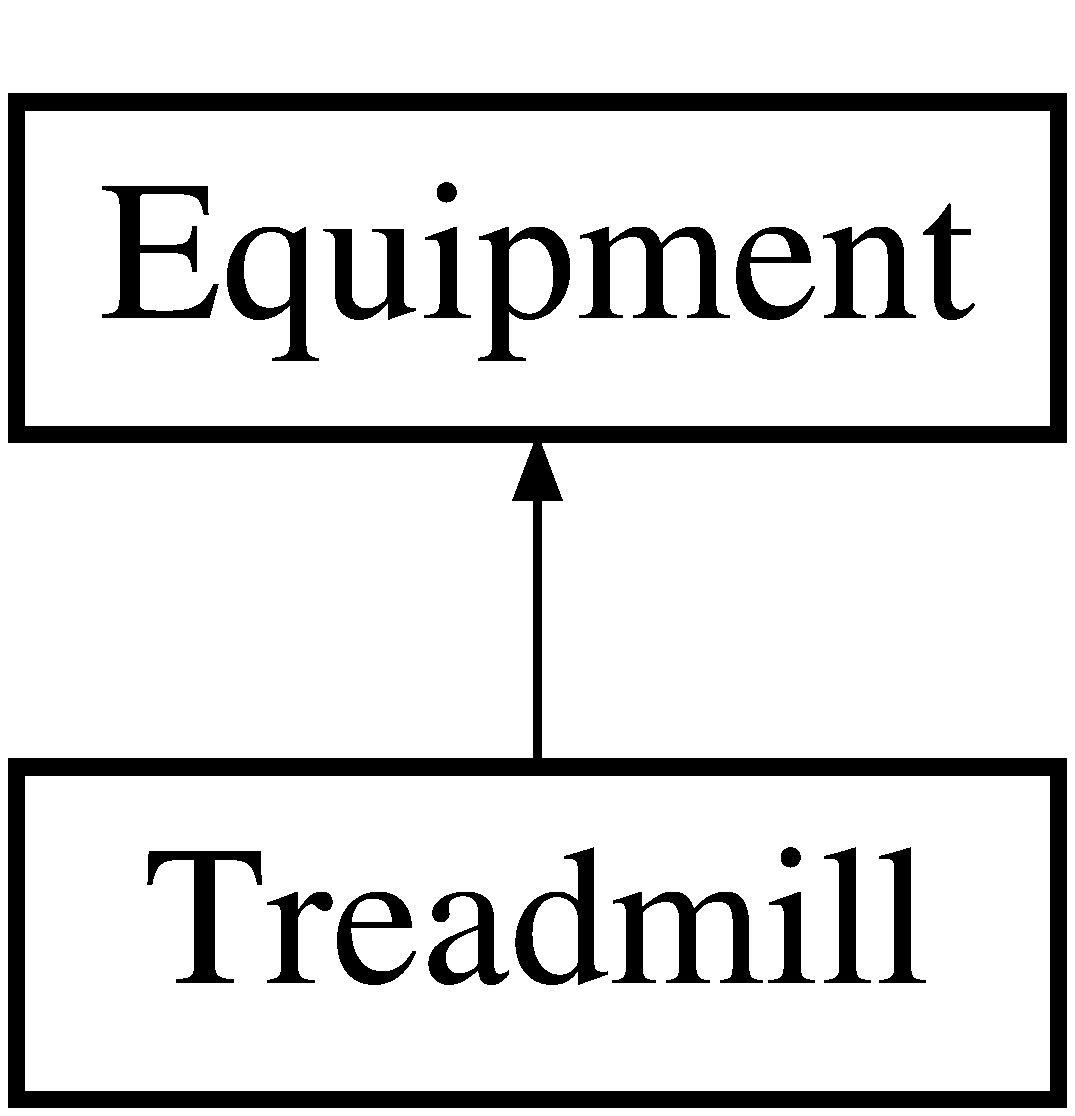
\includegraphics[height=2.000000cm]{class_treadmill}
\end{center}
\end{figure}
\subsection*{Public Member Functions}
\begin{DoxyCompactItemize}
\item 
\hypertarget{class_treadmill_a3104f532767a01da7e48a9935242a032}{}\hyperlink{class_treadmill}{Treadmill} $\ast$ \hyperlink{class_treadmill_a3104f532767a01da7e48a9935242a032}{clone} () const \label{class_treadmill_a3104f532767a01da7e48a9935242a032}

\begin{DoxyCompactList}\small\item\em Create a clone of this piece of equipment at the same state. \end{DoxyCompactList}\item 
\hypertarget{class_treadmill_a62c7b79ca95f62d6ec3720cdaab9cbf0}{}void \hyperlink{class_treadmill_a62c7b79ca95f62d6ec3720cdaab9cbf0}{store} () const \label{class_treadmill_a62c7b79ca95f62d6ec3720cdaab9cbf0}

\begin{DoxyCompactList}\small\item\em Serialize this piece of equipment as J\+S\+O\+N. \end{DoxyCompactList}\item 
\hypertarget{class_treadmill_a695c6c44899532cb3505833f4d6dd031}{}string \hyperlink{class_treadmill_a695c6c44899532cb3505833f4d6dd031}{to\+String} () const \label{class_treadmill_a695c6c44899532cb3505833f4d6dd031}

\begin{DoxyCompactList}\small\item\em Return a string representation of this piece of equipment, in this case \textquotesingle{}\hyperlink{class_treadmill}{Treadmill}\textquotesingle{}. \end{DoxyCompactList}\end{DoxyCompactItemize}


The documentation for this class was generated from the following file\+:\begin{DoxyCompactItemize}
\item 
main.\+cpp\end{DoxyCompactItemize}

%--- End generated contents ---

% Index
\backmatter
\newpage
\phantomsection
\clearemptydoublepage
\addcontentsline{toc}{chapter}{Index}
\printindex

\end{document}
